% Contenidos del capítulo.
% Las secciones presentadas son orientativas y no representan
% necesariamente la organización que debe tener este capítulo.

\section{Introducción}
En los últimos años, el sector del turismo rural ha experimentado un notable crecimiento, motivado por el interés creciente de los viajeros por destinos más tranquilos, naturales y alejados del turismo de masas, según el \gls{ine}~\cite{turismorural:2025}. La Figura~\ref{fig:estadistica} muestra cómo este crecimiento se intensifica sobre todo en las épocas menos señaladas del año, lo que influye en el interés de hacer visible y accesible este tipo de turismo a todo el mundo. Este contexto ha impulsado la digitalización de los servicios ofrecidos por las casas rurales, permitiendo mejorar la experiencia del huésped y optimizar la gestión por parte de los propietarios.

\begin{figure}[h!tb]
    \centering
    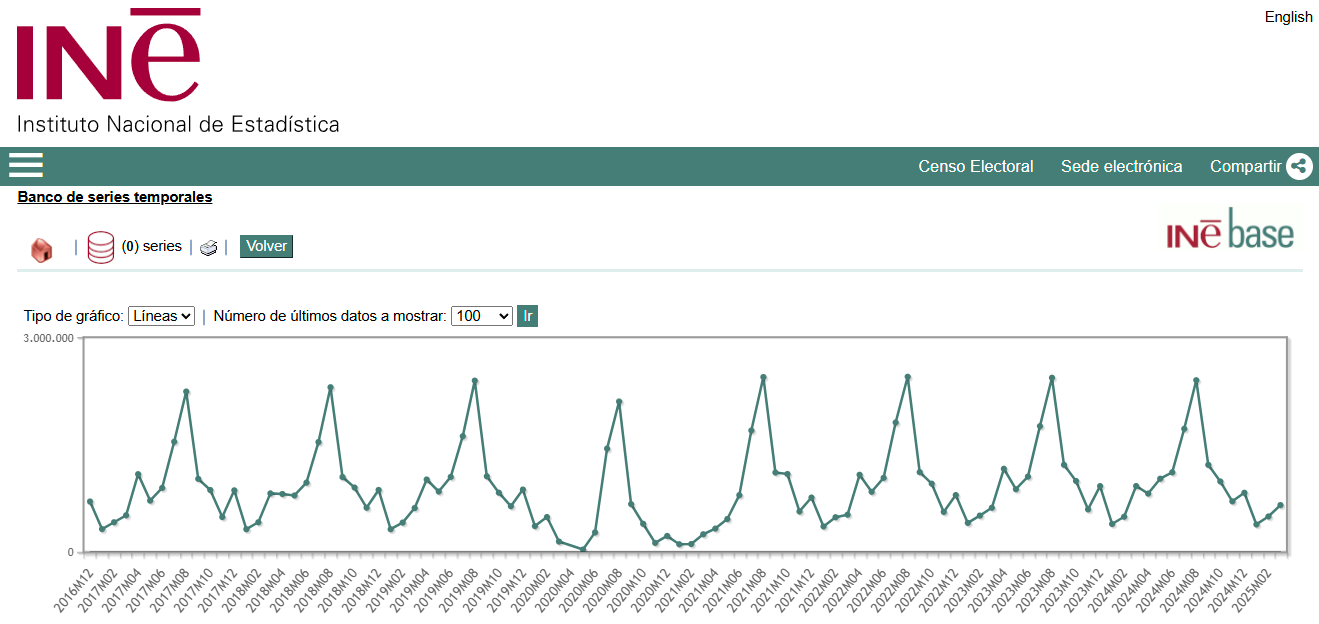
\includegraphics[width=1\textwidth]{figs/turismo-rural.png}
    \caption{Crecimiento del turismo rural en España.}
    \label{fig:estadistica}
\end{figure}

En el presente \gls{tfm}, se va a realizar el desarrollo de una plataforma web para la gestión de una casa rural, ya que, realizando una búsqueda en Google Trends~\cite{g-trends:2025} sobre las poblaciones cercanas a las instalaciones de esta casa rural, se observa en la Figura~\ref{fig:tuejar-turismo} que existe interés por el turismo rural en la zona, especialmente en los meses de verano y durante las festividades. Por lo que se confirma la necesidad de contar con una herramienta que permita gestionar de forma eficiente la promoción del alojamiento.

\begin{figure}[h!tb]
    \centering
    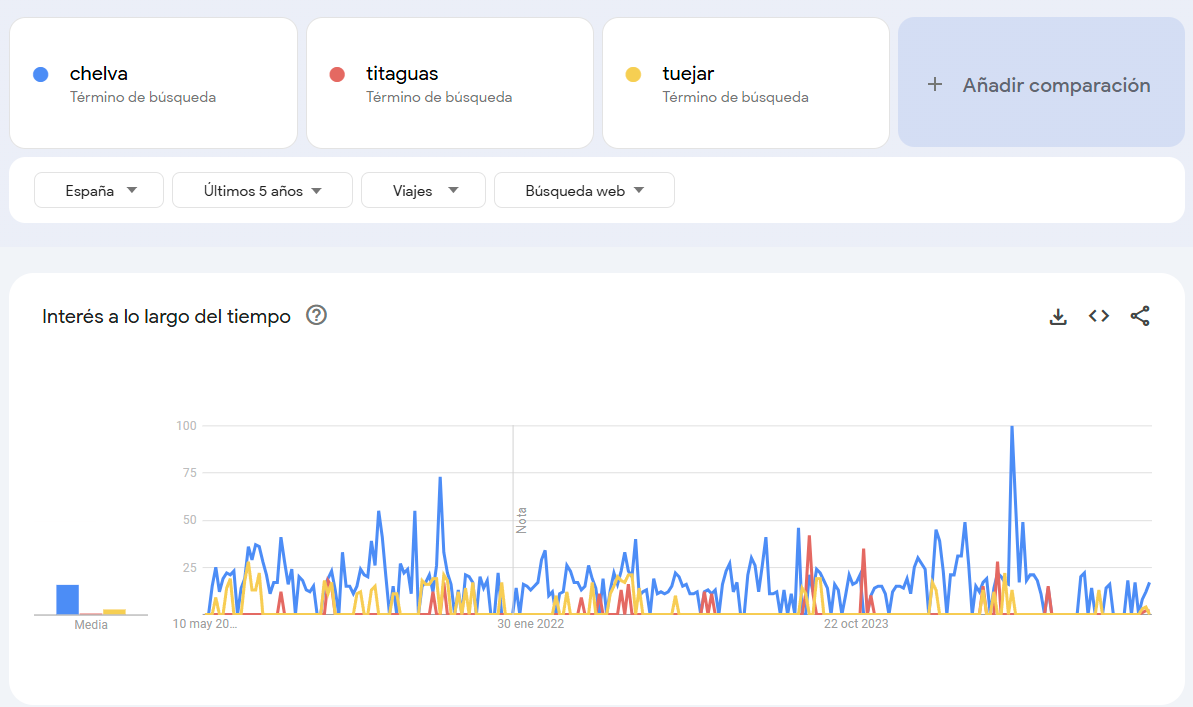
\includegraphics[width=1\textwidth]{figs/turismo-tuejar.png}
    \caption{Interés por el turismo rural en la zona de la casa rural.}
    \label{fig:tuejar-turismo}
\end{figure}

Concretamente, el desarrollo trata la creación de una plataforma web destinada a facilitar la administración y promoción de una casa rural. Esta aplicación, accesible desde dispositivos móviles y navegadores web, tiene como objetivo integrar diferentes funcionalidades: desde la reserva de estancias hasta la sugerencia de actividades turísticas personalizadas, aprovechando tecnologías modernas como los \texttt{microservicios}, bases de datos en la nube y sistemas de recomendaciones inteligentes basados en preferencias del usuario.

La aplicación propuesta incluye múltiples módulos, tales como un calendario de disponibilidad (\texttt{calendar}), recomendaciones contextuales basadas en geolocalización, formularios de contacto y un sistema de reseñas. Todo esto se implementará bajo una arquitectura modular y escalable, siguiendo los principios de diseño orientado a servicios.

Además, se han tenido en cuenta aspectos no funcionales relevantes como la accesibilidad, seguridad de los datos y compatibilidad entre dispositivos. Para garantizar la calidad del software, se utilizarán herramientas como \texttt{Docker} y \texttt{Kubernetes} para el despliegue y orquestación de contenedores, permitiendo una alta disponibilidad y una escalabilidad horizontal efectiva.

Con este trabajo se pretende no solo diseñar una herramienta útil para los propietarios de casas rurales, sino también aportar una visión sobre cómo las tecnologías emergentes pueden transformar el turismo rural, haciéndolo más sostenible, inclusivo y personalizado.

\section*{Motivación}
El presente \gls{tfm} está motivado por diversos factores, tanto personales como técnicos. La motivación principal surge a raíz de una necesidad real: un familiar del autor ha puesto en marcha una casa rural y requiere una aplicación web que le permita gestionar de forma eficiente tanto las reservas como la promoción del alojamiento. Esta situación concreta ofrece una oportunidad ideal para aplicar los conocimientos adquiridos durante el máster en el desarrollo de una solución tecnológica útil, funcional y con aplicación inmediata en un contexto real.

A nivel técnico, este proyecto permite consolidar competencias clave en el ámbito del desarrollo de software moderno, como el diseño de arquitecturas de microservicios, el uso de tecnologías web actuales como Angular y Spring Boot, y la implementación de soluciones escalables y portables mediante contenedores Docker y orquestación con Kubernetes. Estas herramientas permiten construir un sistema distribuido, adaptable a distintos entornos de ejecución y preparado para crecer en funcionalidad en el futuro.

Además, existe un interés adicional en explorar la integración de fuentes de datos externas —como servicios meteorológicos o de eventos turísticos— que aporten valor añadido al usuario final. También se aborda el uso combinado de bases de datos relacionales y no relacionales, con el objetivo de optimizar el almacenamiento y procesamiento de información en función de su naturaleza.

En conjunto, este trabajo no solo representa un reto técnico y una oportunidad de aprendizaje, sino también una propuesta de valor real en el ámbito del turismo rural. El desarrollo de este sistema pretende demostrar cómo la tecnología puede acercarse a entornos tradicionalmente alejados de la digitalización, mejorando su competitividad, sostenibilidad y capacidad de adaptación a las nuevas demandas del mercado.

\section{Objetivos}
\subsection{Objetivo principal}
Aplicar los conocimientos adquiridos en el Máster de \gls{twcam} a la creación de una plataforma web para una casa rural que permita gestionar reservas, ofrecer información turística y mejorar la experiencia del usuario mediante funcionalidades interactivas e integraciones externas basadas en microservicios.

\subsection{Objetivos específicos}
\begin{itemize}
    \item Facilitar la consulta de la disponibilidad y la reserva en línea del alojamiento.
    \item Mostrar información relevante sobre la casa rural y su entorno.
    \item Integrar contenidos multimedia y datos procedentes de fuentes externas.
    \item Permitir la gestión de usuarios con distintos roles y funcionalidades asociadas.
    \item Asegurar compatibilidad con distintos dispositivos y navegadores web.
    \item Incorporar valoraciones, actividades y recomendaciones personalizadas al entorno.
    \item Garantizar la seguridad, escalabilidad y accesibilidad del sistema.
\end{itemize}

\section{Organización de la memoria}

\section*{Capítulo 1: Introducción}
Este capítulo presenta el contexto general del proyecto, así como la motivación personal y técnica que ha llevado a su desarrollo. Se definen el objetivo general y los objetivos específicos que se persiguen con este trabajo. Finalmente, se expone la estructura de la memoria, anticipando brevemente el contenido de los capítulos posteriores.

\section*{Capítulo 2: Estado del arte}
Se realiza un análisis de aplicaciones existentes similares a la propuesta. Además, se evalúan distintas tecnologías disponibles para el desarrollo del proyecto, incluyendo herramientas de frontend, backend, bases de datos, componentes basados en contenedores y servicios en la nube, justificando las elecciones tomadas.

\section*{Capítulo 3: Requisitos, especificaciones, coste, riesgos y viabilidad}
Este capítulo recoge la descripción funcional y no funcional del sistema propuesto, así como las especificaciones técnicas. También incluye una planificación temporal, una estimación de costes, el análisis de riesgos potenciales y un estudio de viabilidad del proyecto.

\section*{Capítulo 4: Análisis}
Se lleva a cabo un análisis detallado del sistema mediante diagramas de casos de uso, clases de primer nivel y secuencia. Esta fase permite establecer una base sólida para el diseño posterior del sistema, identificando los principales actores, funcionalidades y relaciones entre componentes.

\section*{Capítulo 5: Diseño}
Se describe la arquitectura del sistema, dividiéndolo en subsistemas según su funcionalidad: recursos web, publicaciones y previsión del tiempo. Se presentan los diagramas de clases y el modelo de datos, así como los detalles del despliegue y organización de los componentes del sistema.

\section*{Capítulo 6: Implementación y pruebas}
Este capítulo se centra en la implementación técnica de los diferentes módulos del sistema, incluyendo el desarrollo del \gls{frontend}, \gls{backend} y la dockerización para su despliegue. Además, se detallan las pruebas realizadas, tanto unitarias como funcionales, para asegurar el correcto funcionamiento del sistema.

\section*{Capítulo 7: Conclusiones}
Se presentan las conclusiones obtenidas tras la realización del proyecto, así como una revisión de los costes. Finalmente, se propone una línea de trabajo futuro para continuar mejorando el sistema o extender sus funcionalidades.
